\documentclass[a4paper,12pt]{article}

%%% Работа с русским языком
\usepackage{cmap}					% поиск в PDF
\usepackage{mathtext} 				% русские буквы в формулах
\usepackage[T2A]{fontenc}			% кодировка
\usepackage[utf8]{inputenc}			% кодировка исходного текста
\usepackage[english,russian]{babel}	% локализация и переносы

%%% Страница
\usepackage{extsizes} % Возможность сделать 14-й шрифт
\usepackage{geometry} % Создание полей
\geometry{top = 2cm}
\geometry{bottom = 2cm}
\geometry{left = 2.5cm}
\geometry{right = 2.5cm}
\renewcommand{\baselinestretch}{1.5} % Интерлиньяж 1.5

%%% Дополнительная работа с математикой
\usepackage{amsmath,amsfonts,amssymb,amsthm,mathtools} % AMS
\usepackage{icomma} % "Умная" запятая: $0,2$ --- число, $0, 2$ --- перечисление

%% Номера формул
%\mathtoolsset{showonlyrefs=true} % Показывать номера только у тех формул, на которые есть \eqref{} в тексте.
%\usepackage{leqno} % Нумерация формул слева

%% Свои команды
\DeclareMathOperator{\sgn}{\mathop{sgn}}

%% Перенос знаков в формулах (по Львовскому)
\newcommand*{\hm}[1]{#1\nobreak\discretionary{}
	{\hbox{$\mathsurround=0pt #1$}}{}}

%%% Работа с картинками
\usepackage{graphicx}  % Для вставки рисунков
\graphicspath{{images/}{images2/}}  % папки с картинками
\setlength\fboxsep{3pt} % Отступ рамки \fbox{} от рисунка
\setlength\fboxrule{1pt} % Толщина линий рамки \fbox{}
\usepackage{wrapfig} % Обтекание рисунков текстом

%%% Работа с таблицами
\usepackage{array,tabularx,tabulary,booktabs} % Дополнительная работа с таблицами
\usepackage{longtable}  % Длинные таблицы
\usepackage{multirow} % Слияние строк в таблице

%%% Теоремы
\theoremstyle{plain} % Стиль по умолчанию
\newtheorem{theorem}{Теорема}[section]
\newtheorem{proposition}[theorem]{Утверждение}

\theoremstyle{definition} % "Определение"
\newtheorem{corollary}{Следствие}[theorem]
\newtheorem{problem}{Задача}[section]

\theoremstyle{remark} % "Примечание"
\newtheorem*{nonum}{Решение}

%%% Программирование
\usepackage{etoolbox} % логические операторы

\usepackage{lastpage} % Узнать, сколько всего страниц в документе.

\usepackage{soul} % Модификаторы начертания

\usepackage{graphicx} %Подключаю модули для добавления картинок
\graphicspath{.}
\DeclareGraphicsExtensions{.pdf,.png,.jpg}




	
	\renewcommand{\baselinestretch}{1.5}
	
	\begin{document}
		\renewcommand{\contentsname}{\Large Содержание}
		\renewcommand{\bibname}{\normalfont\Large\bfseries Список литературы}
		
		\begin{titlepage}
			\begin{center}
				Министерство науки и высшего образования Российской Федерации \\
				НАЦИОНАЛЬНЫЙ ИССЛЕДОВАТЕЛЬСКИЙ ЯДЕРНЫЙ УНИВЕРСИТЕТ <<МИФИ>> \\*
				\hrulefill
			\end{center}
		
		\begin{center}
			ИНСТИТУТ ЛАЗЕРНЫХ И ПЛАЗМЕННЫХ ТЕХНОЛОГИЙ\\
			КАФЕДРА №31 ПРИКЛАДНАЯ МАТЕМАТИКА
		\end{center}
		\vspace{1cm}
		
		\vspace{2em}
		
		\begin{center}
			\large{Отчет}
			
			по проектной практике на тему:
		\end{center}
		
		\begin{center}
			\large "Изучение навыков работы в программе SALOME. Изучение работы с командами консоли. Написание скриптов для SALOME на языке Python."
	

		\textit{Авторы: Есис А. И., Павленок Л. Л.}
		
		\textit{Руководитель проекта: Чмыхов М. А.}
		\end{center}
	
	

\vspace{26em}
		
		\begin{center}
			г. Москва 2020
		\end{center}
	\end{titlepage}

	\newpage 
	\tableofcontents
	\setcounter{page}{3}
	
	\newpage
	\section*{Аннотация}
	
	3D-моделирование стало неотъемлемой частью нашей жизни. Сегодня оно широко используется в сфере маркетинга, архитектурного дизайна и кинематографии, не говоря уже о промышленности. 3D-моделирование позволяет cоздать прототип будущего сооружения, коммерческого продукта в объемном формате.
	
	Cегодня невозможно представить 2 крупные отрасли без применения трехмерных моделей. Это — промышленность и индустрия развлечений.
	С индустрией развлечений мы сталкиваемся почти каждый день. Это фильмы, анимация и компьютерные игры. С помощью одного и того же принципа — полигонального моделирования cозданы многие виртуальные миры и персонажи. Полигональное моделирование происходит путем манипуляций с полигонами в пространстве. Вытягивание, перемещение вращение,  и.т.д. Однако невозможно контролировать необходимые зазоры, сечения, учесть физические свойства материала и технологию изготовления, используя полигональное моделирование. Для таких изделий используются методы промышленного проектирования.

	Цель проекта: Научить работать с визуальныйм интерфейсом программе Salome и строить 3D модели при помощьPython скриптов; строить расчетную сетку моделей и моделирование поведения объектов в разных ситуациях.

	Задачи: 
	\begin{enumerate}
	\item Научиться роботать с визуальным интерфейсом программмы SALOME
	\item Построить 3D модели с помощью визуального интерфейса программы SALOME
	\item Построить 3D модели с помощью Python скриптов
	\item Наожить сетку на изучаемую модель
	\item Построить Математическую модель исследуемого объекта и предсказать его поведение в различных средах
	\end{enumerate}
	
	\newpage
	\section{Проделанная работа}
	
	На данном этапе этапе выполнения проета была изучена литература, на основании которой был составлен следующий обзор:
	CAПР (Система Aвтоматизированного Поектирования). Современные CAD-подсистемы, входящие в состав интегрированных САD/CAM/CAE-систем — поддержанное компьютером конструирование/изготовление/ инженерная деятельность), и системы твердотельного параметрического моделирования механических объектов, отражающие последние достижения инженерной компьютерной графики, представляют собой наиболее важные разработки в области новых технологий по автоматизации деятельности инженеров,	конструкторов и технологов. По уровню возможностей САПР условно разделяются на три уровня:
	\begin{enumerate}
		\item САПР нижнего уровня — это, чаще всего, программы для двумерного проектирования.
		\item САПР среднего уровня — позволяют дополнительно создавать трехмерные параметрические модели и выполнять проверочные расчеты деталей и сборок.
		\item САПР верхнего уровня — обеспечивают потребности практически всех областей проектирования, от разработки изделий и оснастки до проведения сложных инженерных расчетов и изготовления изделий\cite{bBolshakov}.
	\end{enumerate}
	В данной работе мы используем САПР среднего уровня, которой является Salome-MECA. Изначально задуманная в качестве связующего ПО CAD-CAE, она включает в себя разнообразные модули, используемые в приложениях численного моделирования — от моделирования в САПР до параллельных вычислений. Одним из важнейших преимуществ Salome-MECA является то, что её исходный код открыт и бесплатно распространяется на условиях GNU Lesser General Public License. Это означает, что Salome может расширяться за счет сторонних свободных или коммерческих модулей. Внутренним языком платформы является Python, причем в самой платформе имеется встроенная консоль, которая может быть использованна для выполнения пользовательских сценариев и автоматизации обработки множества типовых задач (пакетной обработки)\cite{wOfDoc}. Платформа Salome, как и любая CAE-система, состоит из четырех модулей: решателя (Solver), поcтроителя сетки (Mesh), модуля поcтроения геoметрии (Geometry), модуля oбработки и представления результатов (Pоst-processing).
			
	 Метод конечных элементов лежит в основе некоторых CAE-пакетов . Идея этого метода заключается в замене непрерывной функции, описывающей изучаемое явление или процесс, дискретной моделью, которая строится на базе множества кусочно-непрерывных функций, определенных на конечном числе подобластей. Каждая такая подобласть конечна и представляет собой часть (элемент) всей области, поэтому их называют конечными элементами. Иcследуемая геометрическая область разбивается на элементы так, чтобы на каждом из них неизвестная функция аппроксимировалась пробной функцией. Такое разбиение называется расчетной сеткой. Создание хорошей расчетной сетки также представляет собой нетривиальную задачу. Это связано с тем, что реальные детали машин имеют сложную геометрию и необходимо разделить их на такие элементы, чтобы приближенные решения не сильно отличались от точных. Поэтому, кроме самих CAE-пакетов, существует бoльшое число приложений, выполняющих всего одну важную функцию: построение расчетной сетки \cite{wIbmSalome}. В данной работе наибольший интерес представляют модуль Geometry и Mesh, поскольку для них предусмотренно написание скриптов.
	
	Любая задача моделирования начинается с создания геометрической модели изучаемого объекта – определения его формы. Другими cловами, необходимо задать границы той части пространства, поведение которой необходимо исследовать. Геометрическая модель может представлять собой двумерный или трехмерный чертеж.
		
	Геометрический модуль SALOME разработан для:
	\begin{itemize}
		\item Построения и оптимизации геометрических моделей, используя широкий набор функций автоматизированного проектирования
		\item Создание элементарных геометрических объектов
		\item Поcтроение примитивов
		\item Построение форм
		\item Генерирование сложных форм
		\item Работа c группами
		\item Геометрические булевы (логические) операции
		\item Геометрические преобразования
		\item Построение блоками
	\end{itemize}
	
	В геометрический модуль можно как экспортировать, так и импортировать геометрические объекты следующих форматов: BREP, IGES, STEP. Механизмы импорта и экспорта осуществлены через дополнения (плагины), что дает возможность расширить диапазон доступных форматов, добавляя другие приложения-дополнения (плагины) (такие как CATIA 5)\cite{wLadugaGeom}.
	
	Любой реальный исследуемый объект чаще всего обладает достаточно сложной формой. И описать его поведение при наложении внешних нагрузок, как цельное, достаточно сложно хотя бы потому, что любой объект чаще всего имеет в своем составе хотя бы несколько элементов. Следовательно, нужно записать точные математические выражения для граничных условий на поверхности каждого типа, а затем совместить их.
		
	Можно использовать другой алгоритм, разбивая всю деталь на очень мелкие фрагменты определенной формы (конечные элементы): треугольники, четырехугольники, шестиугольники и т.д. для 2D-объектов и тетраэдры, гексаэдры и т.д. для 3D-объектов. Граничные условия для каждого такого фрагмента будут иметь достаточно простой вид. Более того, из-за малых размеров элемента, решение для него можно аппроксимировать при помощи элементарных функций, например, линейным или квадратичным полиномом. Используя данный алгоритм, мы получим систему алгебраических уравнений, для решения которой существует большое количество легко реализуемых методов.
		
	При разбиении объекта на малые элементы сначала необходимо определить точки, которые будут вершинами элементов. Эти точки называют узлами (node) расчетной сетки или 0D-элементами. Далее, на основе выбранных алгоритмов и геометрии базовых элементов, узлы соединяются прямыми линями, называемыми ребрами (edge) или 1D-элементами. Область, заключенная между несколькими ребрами и не содержащая ни одного узла или ребра, называется гранью (face) или 2D-элементом. Обычно грани образуются тремя или четырьмя ребрами. Область, заключенная между несколькими гранями и не содержащая ни одного узла, ребра или грани (части грани) называется объемным (volume object) или 3D-элементом.
		
	Разбиение объекта на элементы в Salome выполняется по выбираемым пользователем алгоритмам и на основе параметров, оформляемых в виде гипотез \cite{wIbmSalomeMesh}.
		
	Модуль MESH SALOME предназначен для\cite{wOfDoc}:
	\begin{itemize}
		\item Импорта и экспорта сеток в формате MED
		\item Сцепление геометрических моделей, ранее созданных или импортированных компонентом Geometry
		\item Модификации в местном масштабе сгенерированных сеток
		\item Суммирования узлов и элементов (Addition of nodes and elements)
		\item Удаления узлов и элементов (Removal of nodes and elements)
		\item Контроля качества сеток, базирующихся на ряде определенных критериев
	\end{itemize}

	Чего нам удалось добиться в ходе выполнения проекта:
	Были построены 3D модели различных деталей различной сложности, что позволило научиться пользоваться визуальным интерфейсом программы. Модели строились по возрастанию сложности. от простых геометрических объектов, таких как куб, цилиндр и т. д. до сложных фигур включающих в себя множество простых объектов. Сложные детали были смоделированны по изображению детали с задаными размерами. 

Простые модели:




	\begin{figure}[h]
		\begin{center}
			\begin{minipage}[h]{0.4\linewidth}
				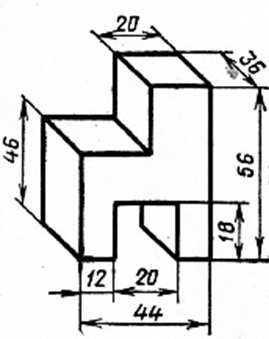
\includegraphics[width=1\linewidth]{17.1}
				\caption{Рисунок модели} %% подпись к рисунку
			\end{minipage}
			\hfill
			\begin{minipage}[h]{0.4\linewidth}
				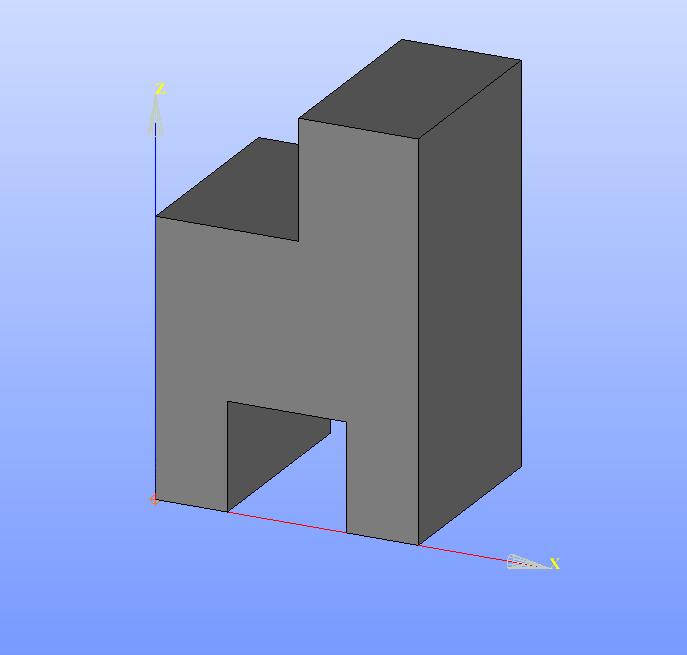
\includegraphics[width=1\linewidth]{17.12}
				\caption{Модель}
			\end{minipage}
		\end{center}
	\end{figure}
\newpage

Сложные модели:

	\begin{figure}[h]
		\begin{center}
			\begin{minipage}[h]{0.4\linewidth}
				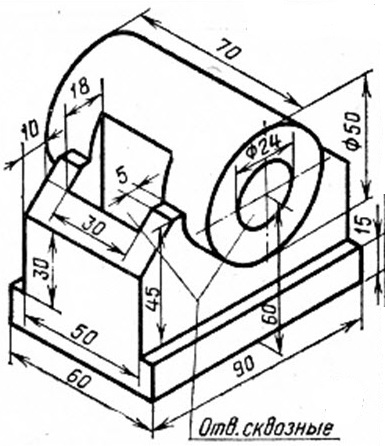
\includegraphics[width=1\linewidth]{17.3}
				\caption{Рисунок модели} %% подпись к рисунку
			\end{minipage}
			\hfill
			\begin{minipage}[h]{0.4\linewidth}
				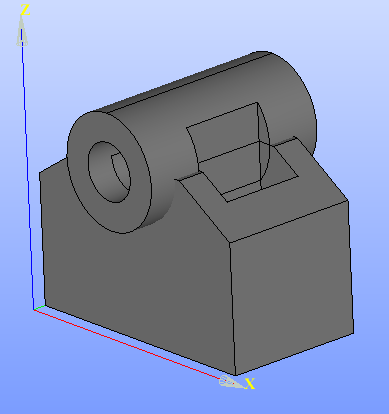
\includegraphics[width=1\linewidth]{17.32}
				\caption{Модель}
			\end{minipage}
		\end{center}
	\end{figure}

Далее мы приступили к построению моделей с помощью Python скриптов. Это более сложная и интересная задача, с синтаксисом языка мы были ознакомлемы, поэтосу с этим проблем не вознникло. Сначало мы исследовали уже построеенные детали, смотрели как они выглядят в виде Python скрипта, после чего начали сами эксперементировать, что заняло много времени, но это было необходимо, так как дальнейшая работа основывалась на этом. Переходя от простых деталей к более сложным нам удалось достигнуть результата и мы научились строить модели деталей скриптами. Построение детали скриптами позволяет автоматизировать многие вещи и экономит время.


С помощью данного кода из скрипта

\begin{verbatim}

geompy = geomBuilder.New()
O = geompy.MakeVertex(0, 0, 0)
OX = geompy.MakeVectorDXDYDZ(1, 0, 0)
OY = geompy.MakeVectorDXDYDZ(0, 1, 0)
OZ = geompy.MakeVectorDXDYDZ(0, 0, 1)
Box_2 = geompy.MakeBoxDXDYDZ(9, 30, 18)
Box_3 = geompy.MakeBoxDXDYDZ(23, 30, 38)
Box_4 = geompy.MakeBoxDXDYDZ(9, 10, 38)
Translation_1 = geompy.MakeTranslation(Box_4, 14, 10, 0)
Cut_1 = geompy.MakeCutList(Box_3, [Translation_1], True)
Translation_2 = geompy.MakeTranslation(Cut_1, 42, 0, 0)
Box_1 = geompy.MakeBoxDXDYDZ(65, 30, 12)
Translation_3 = geompy.MakeTranslation(Box_4, 56, 10, 0)
Cut_2 = geompy.MakeCutList(Box_1, [Translation_3], True)
geomObj_1 = geompy.MakeVertex(-0, -0, 0)
geomObj_2 = geompy.MakeVertex(0, -0, 0)
geomObj_3 = geompy.MakeVertex(0, 0, 0)
geomObj_4 = geompy.MakeVertex(-0, 0, 0)
geompy.addToStudy( O, 'O' )
geompy.addToStudy( OX, 'OX' )
geompy.addToStudy( OY, 'OY' )
geompy.addToStudy( OZ, 'OZ' )
geompy.addToStudy( Box_4, 'Box_4' )
geompy.addToStudy( Translation_3, 'Translation_3' )
geompy.addToStudy( Box_2, 'Box_2' )
geompy.addToStudy( Box_3, 'Box_3' )
geompy.addToStudy( Translation_1, 'Translation_1' )
geompy.addToStudy( Cut_1, 'Cut_1' )
geompy.addToStudy( Translation_2, 'Translation_2' )
geompy.addToStudy( Box_1, 'Box_1' )
geompy.addToStudy( Cut_2, 'Cut_2' )

\end{verbatim}
\newpage




	\begin{figure}[h]
		\center{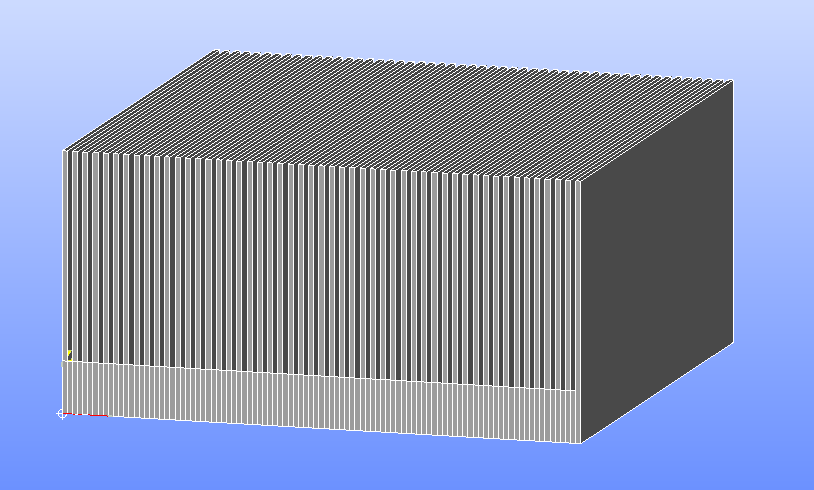
\includegraphics[width=30em]{1}}
		\caption{Можно построить такую фигуру}
	\end{figure}
	
После того, как мы научились строить 3D модели деталей, мы перешли к накладыванию сетки. Возникли сложности с подбором таких параметров, как: Параметры гипотезы, параметры разбиения. Но поле нескольких эксперементов стало поянтнокак подбирать данные параметры.
И наконец мы смогли перейти к построению сайтой математической модели. На донном этапе мы столкнулись с проблемой отсутсвия софда для ОС Windows, решили эту проблему поставив ОС Linux на виртуальную машу и запустив моделирование. Моделировали распростронение тепла в твердом теле с учётом тепловых потерь. В качество твердого тела была взята кастрюла, и смоделированно распростронение тепла от горячего корпуса к ручкам. Результаты проделанной работы можно увидеть на картинках ниже:
\newpage
	\begin{figure}[h]
		\begin{center}
			\begin{minipage}[h]{0.4\linewidth}
				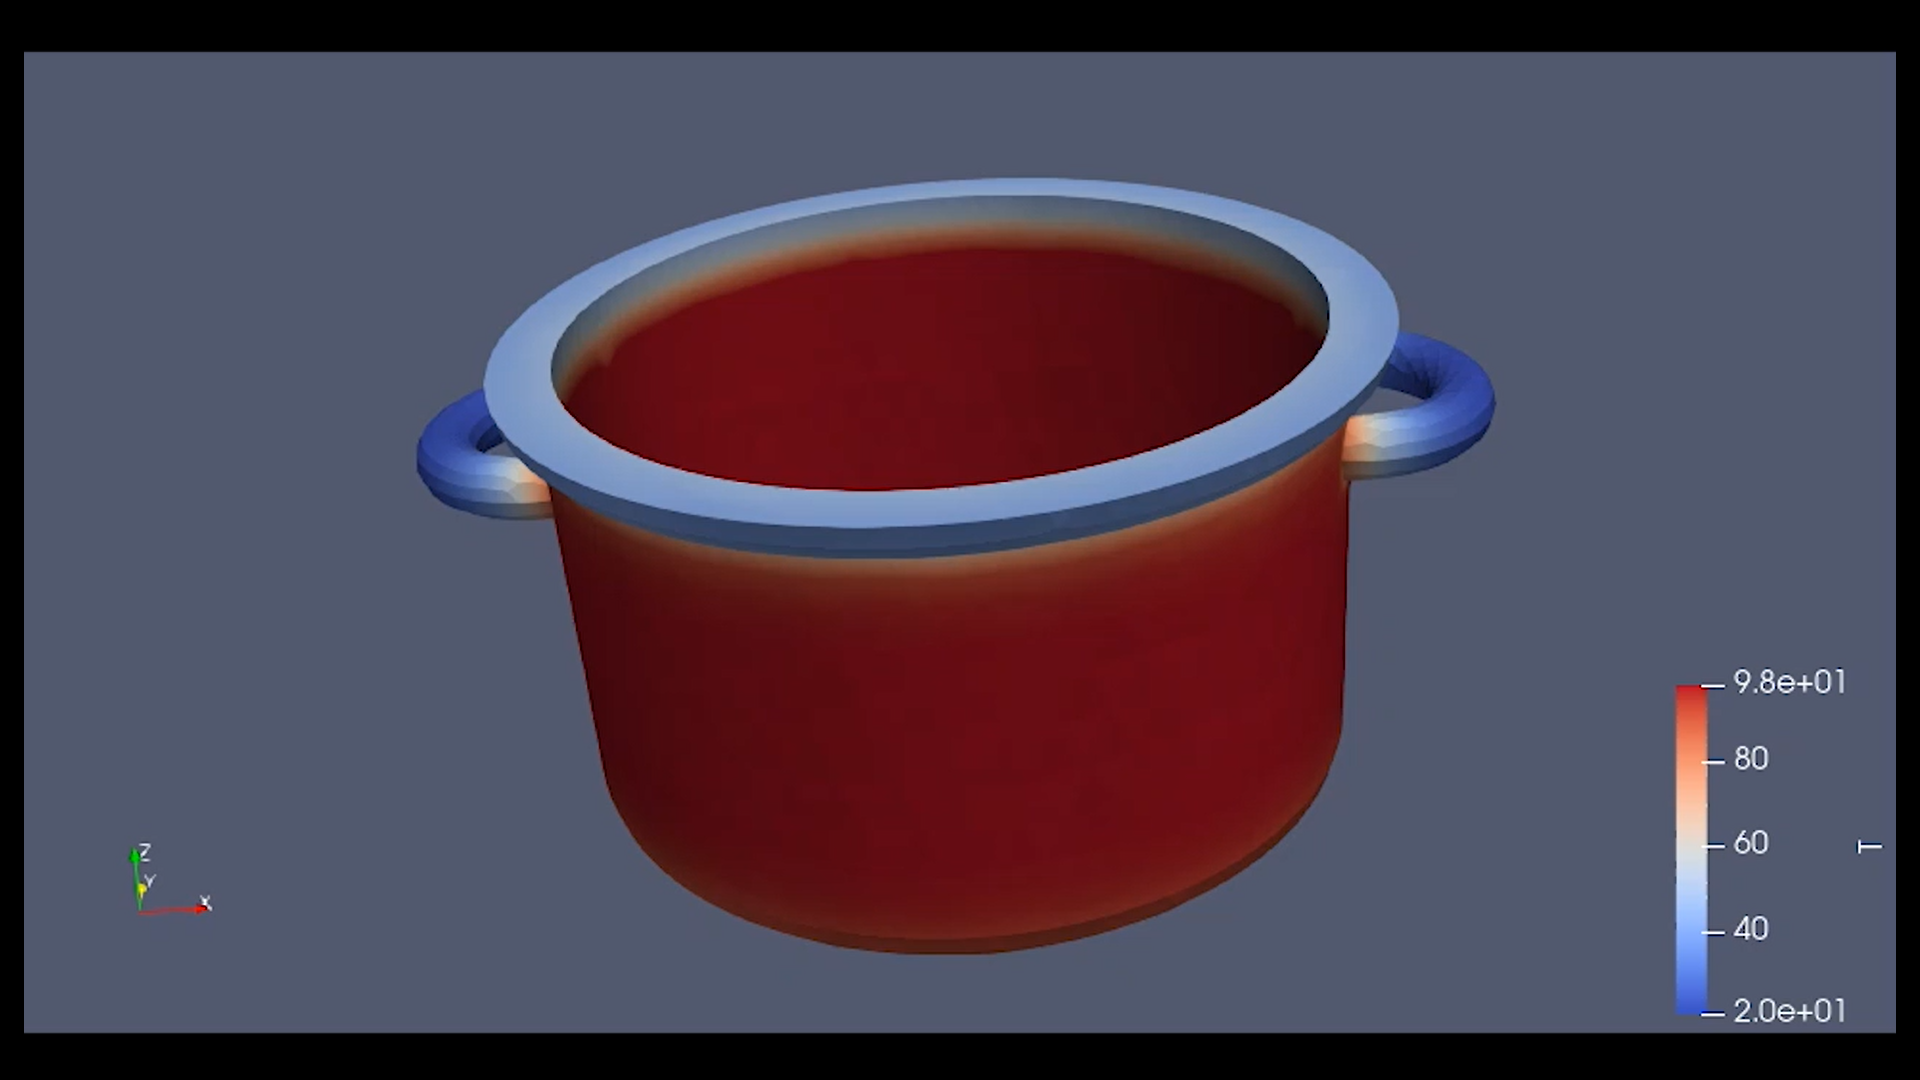
\includegraphics[width=1\linewidth]{1s}
				\caption{1я секунда} %% подпись к рисунку
			\end{minipage}
			\hfill
			\begin{minipage}[h]{0.4\linewidth}
				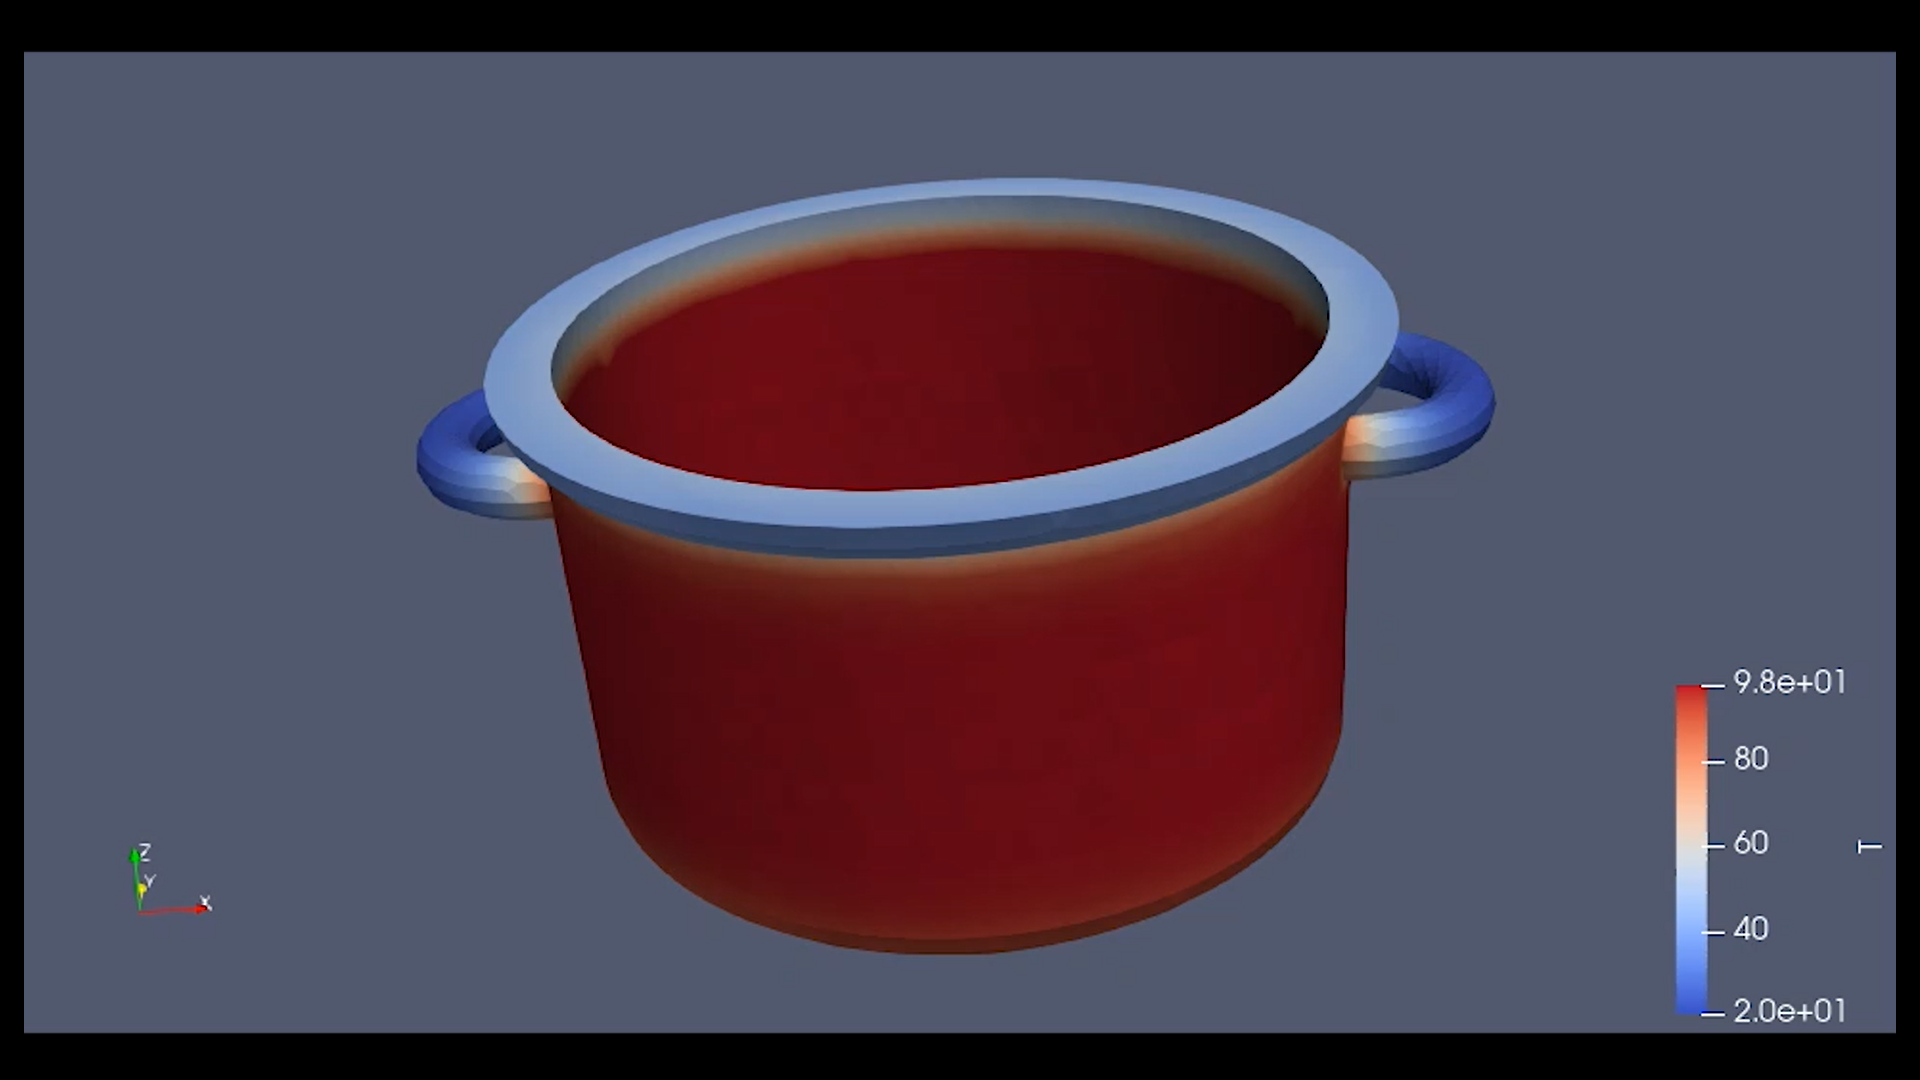
\includegraphics[width=1\linewidth]{2s}
				\caption{5я секунда}
			\end{minipage}
			\begin{minipage}[h]{0.4\linewidth}
				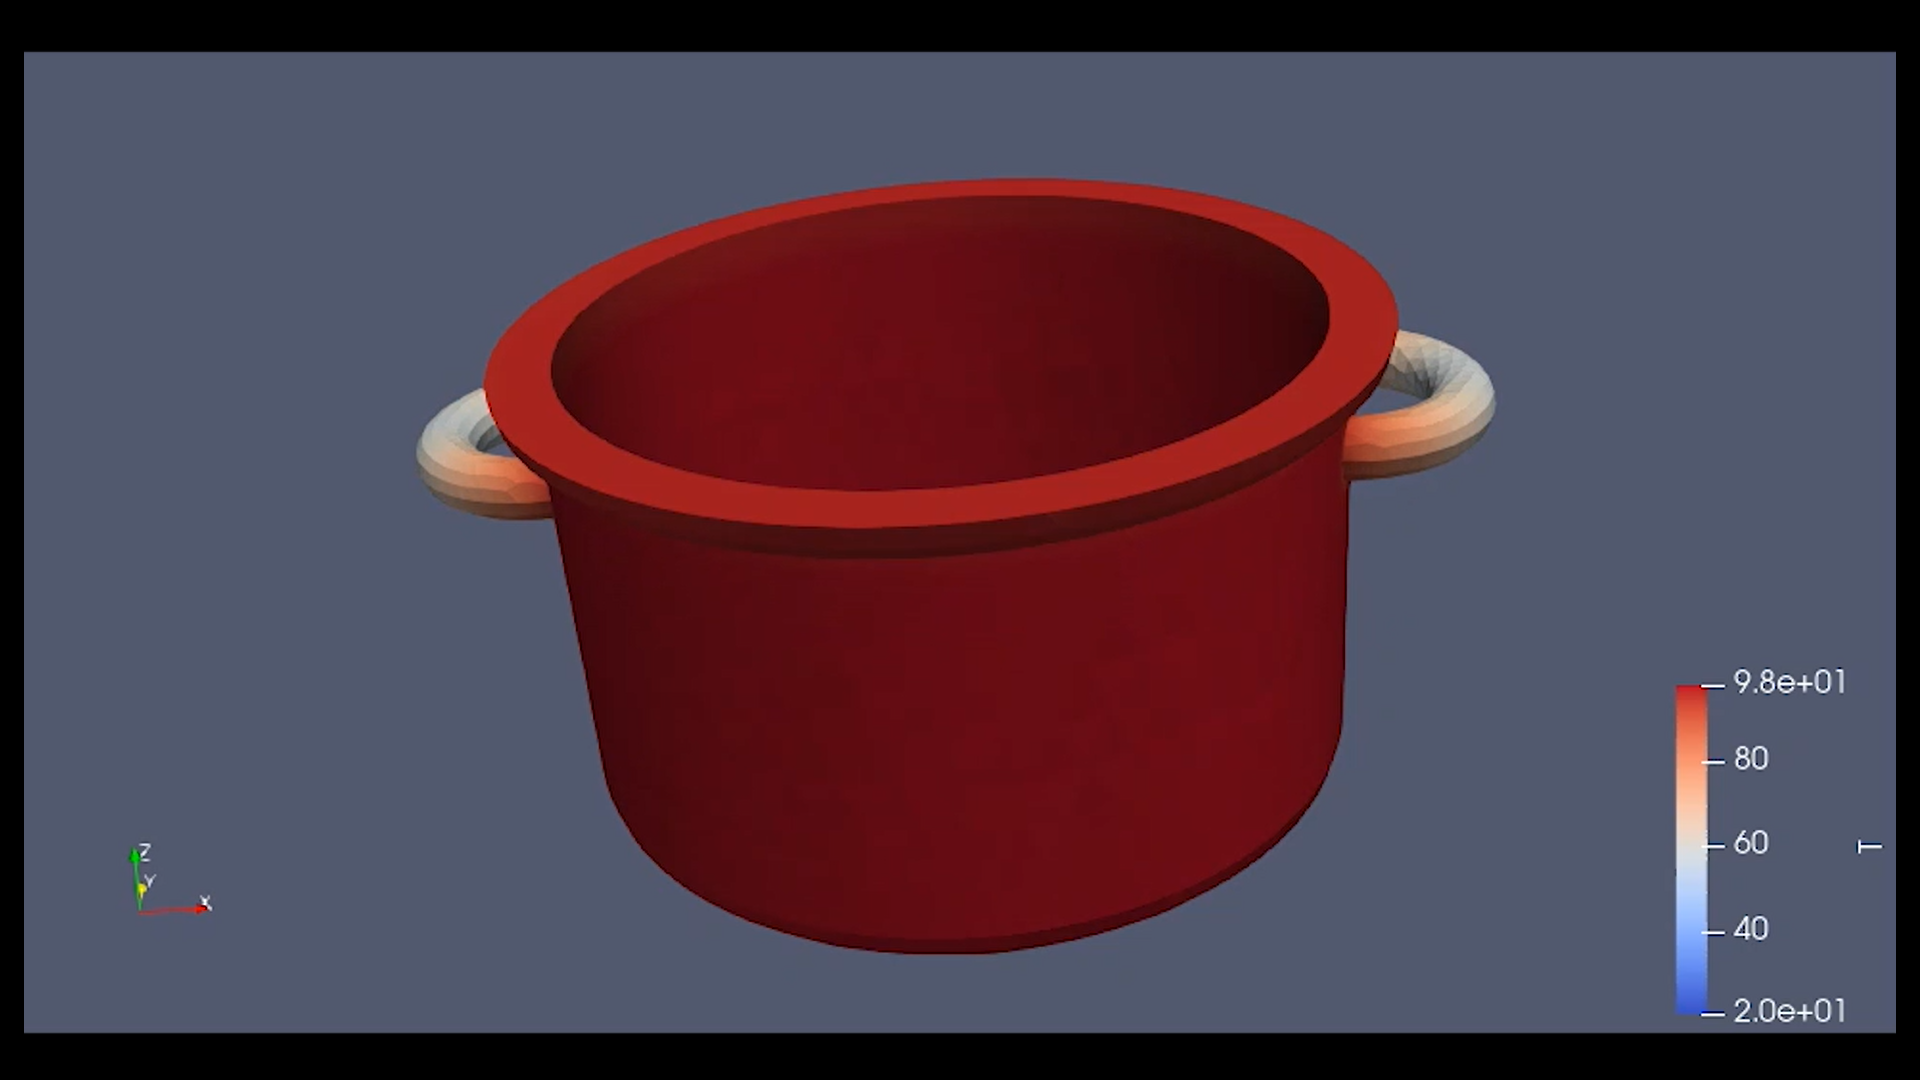
\includegraphics[width=1\linewidth]{3s}
				\caption{10я секунда} %% подпись к рисунку
			\end{minipage}
			\hfill
			\begin{minipage}[h]{0.4\linewidth}
				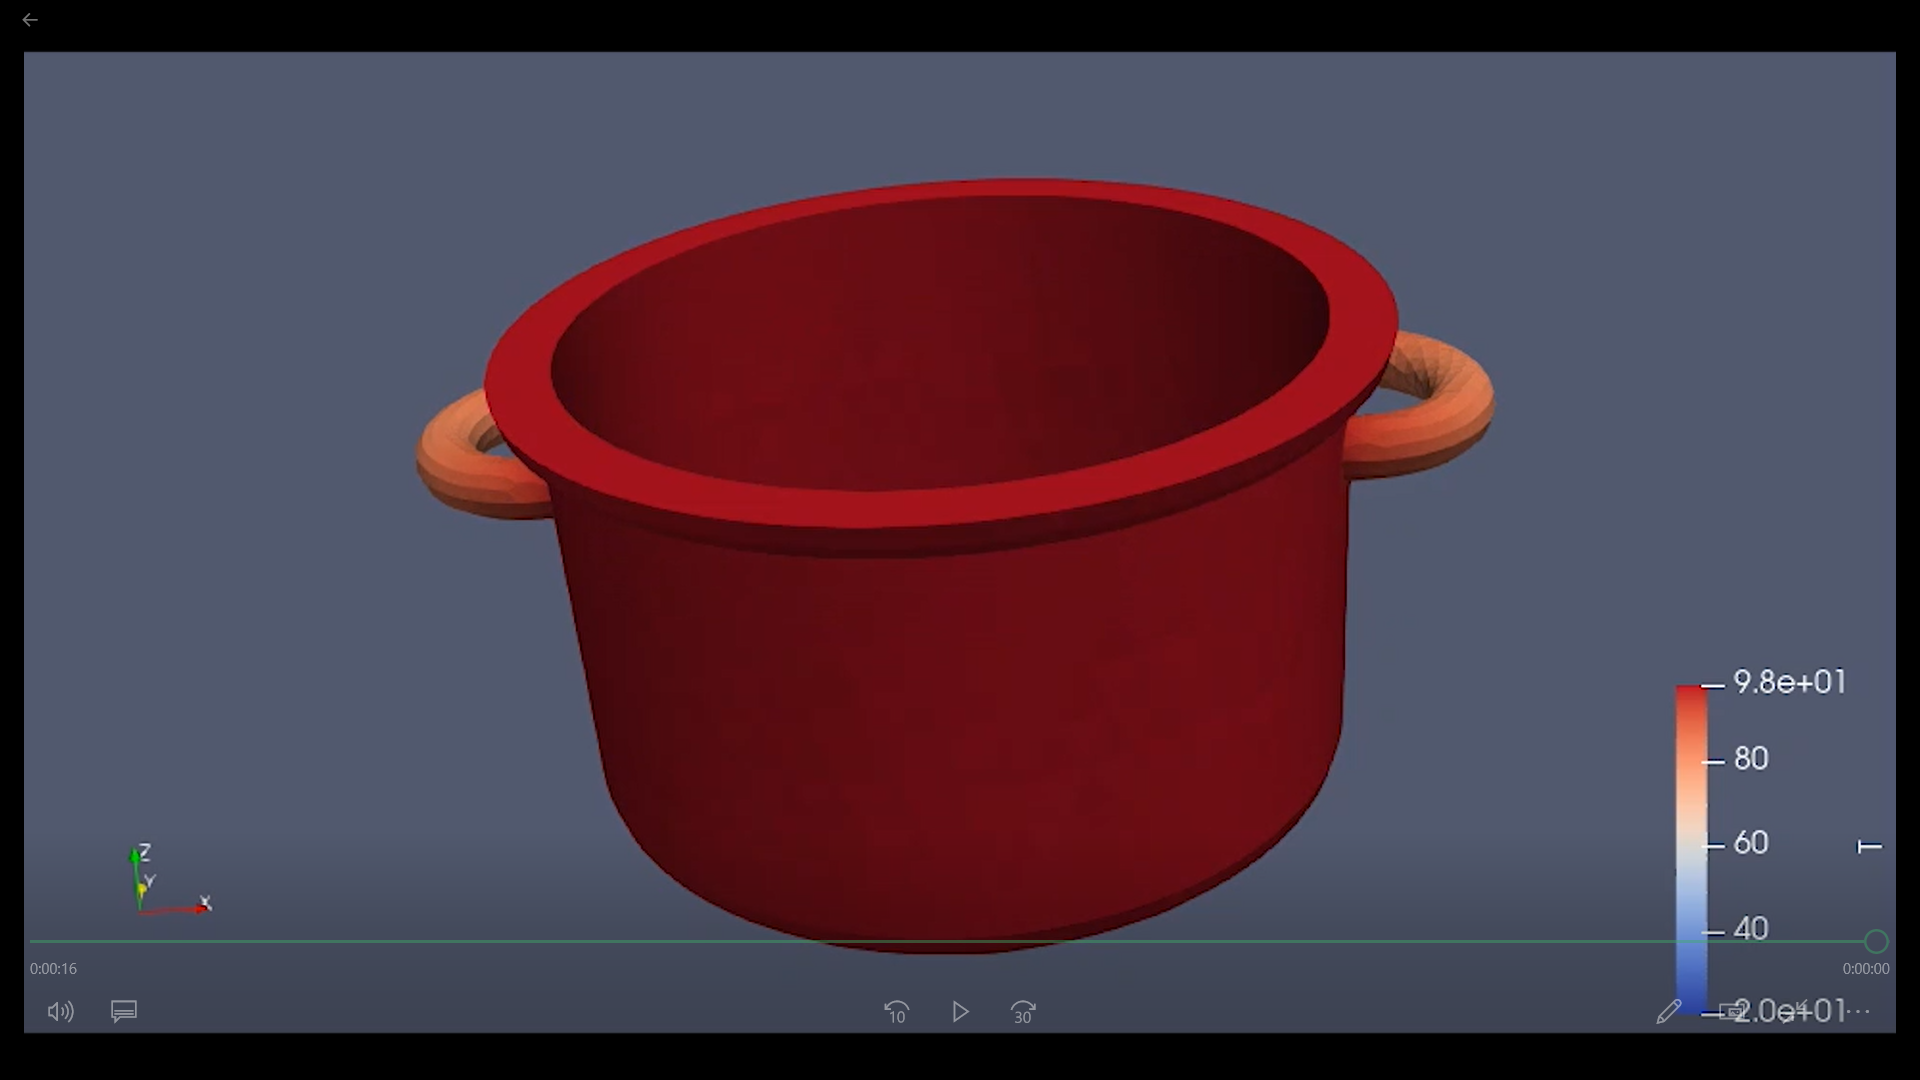
\includegraphics[width=1\linewidth]{4s}
				\caption{15я секунда}
			\end{minipage}
		\end{center}
	\end{figure}

В ходе работы мы использовали систему контроля версий GitHub, что было очень удобно для работе в паре. Так же использовали программу для управления библиографической инфомацией "Mendeley", в ней хранится вся найденная литература по нашей теме, которую в будущем мы сможем использовать для расширения нашего проекта.
\newpage

\section{Дальнейшая работа}
В дальнейшей работе  планируется научится накладывать сетку и строить мат. модели без использования визуального интерфейса, а только при помощь Python скриптов. Наша конечная цель создать модель которая будет строить оптимальную форму радиатора, находящегося в жидкой среде, учитывая характер движения жидкости, ее вязкость и колличество. В качестве алгоритма подбора оптимальной формы планируется использовать генетические алгоритмы.


	\newpage

	\begin{thebibliography}{w:40}
		
		\bibitem{label1} Боргояков Е. А., Кособрюхова О.В. "Современные подходы в профилактике неинфекционных заболеваний". - Ачинск. - 2016.
		
	\end{thebibliography}
	
	\end{document}